\subsection{Logistic Regression}
As a baseline, we first tried a Logistic Regression model. As the algorithm assumes that the features follow a Gaussian distribution, we scaled numerical features using PowerTransformer, which reduces skewness and stabilizes variance.

\subsubsection{Rating}
Using the default parameters yielded a macro F1 of 0.144 and an accuracy of 0.388. We performed a grid search using 5-fold cross validation, which resulted in a very small increase, with a 0.146 average macro F1 on the validation sets and 0.152 on the training set, which at least proves no overfitting.
We tested the following hyperparameters (the values for the final model are in bold):
\begin{lstlisting}[basicstyle=\footnotesize\ttfamily,
                   escapeinside={(*@}{@*)}]
  { 'penalty': [(*@\textbf{'l2'}@*), 'l1', 'elasticnet'],
    'C': [0.001, 0.01, 0.1, 1, (*@\textbf{10}@*), 100],
    'l1_ratio': [0.1, 0.3, 0.5, 0.7, 0.9],
    'solver': ['lbfgs', 'sag', 'saga', 'newton-cg',
        (*@\textbf{'newton-cholesky'}@*), 'liblinear']  }
\end{lstlisting}

On the test set, the final model achieved a \textbf{macro F1} of\textbf{ 0.145} and an \textbf{accuracy} of \textbf{0.388}, comparable to the default model. The poor performances across decision thresholds are confirmed by the \textbf{PR AUC} of only \textbf{0.193}.

The model has managed to generalize some information only for the classes with the highest support: the performances peak for the mode, (7,8] (F1: 0.544), its neighboring classes are confused for it most of the time, and as we move to the tail of the bell distribution, it achieves consistently poor results (F1 < 0.05).

Looking at the model's coefficients, the overall most important feature is \textit{hasCriticReviews} (mean absolute value > 1.2, while for the other coefficients in the top 15 is in the interval [0.6, 0.7]): it is the first or second-biggest coefficient for the best performing classes (i.e. for the interval (5,8]), and for all of them it takes on a negative value, i.e. having critical reviews lowers the probability of a record of having an 'average' rating.

\subsubsection{Title Type}
For this task, the final model resulting from the grid search achieved an average validation macro F1 of 0.653 (on the training set: 0.664). The final parameters chosen were: \texttt{{'C': 100, 'penalty': 'l2', 'solver': 'newton-cg'}}.

On the test set, the model achieved a \textbf{macro F1} of \textbf{0.649} and an accuracy of \textbf{0.908}; the improvement w.r.t. the default parameters (0.647 and 0.908) is, again, quite small. The \textbf{PR AUC} is \textbf{0.704}; the curve for each class reflects its performance.

Given that both tasks have 10 target classes, our intuition about \textit{titleType} yielding better results is confirmed.

The four most popular classes (\textit{tvEpisode}, \textit{short}, \textit{movie}, \textit{tvSeries}) achieve great results, with F1 > 0.9. The best performing and most popular class, \textit{tvEpisode}, peaks with 0.978. All other classes (except \textit{tvShort}) achieve a F1 score > 0.4, which is still significantly more than random chance. \textit{Videogame}, in spite of its low support, manages to achieve very good results (F1 0.76).

The 15 most important features are reported in Fig. \ref{fig:LR_feat_impo_tt.png}. Overall, the two most informative features are:
\begin{itemize}
    \item \textit{canHaveEpisodes}: it has very high positive values for \textit{tvSeries} (+13.15) and \textit{tvMiniSeries} (+12.18) and negative for all other classes; it's also the most important feature for \textit{movie} (-4.75). 
    \item genre \textit{Short}: of course, it's the most important feature for \textit{short} and \textit{tvShort}, and it's the second most important for \textit{video} with positive values; it's high up in the ranking with a negative value for \textit{movie}, \textit{tvEpisode}, \textit{tvMovie}.
\end{itemize}

\begin{figure}
    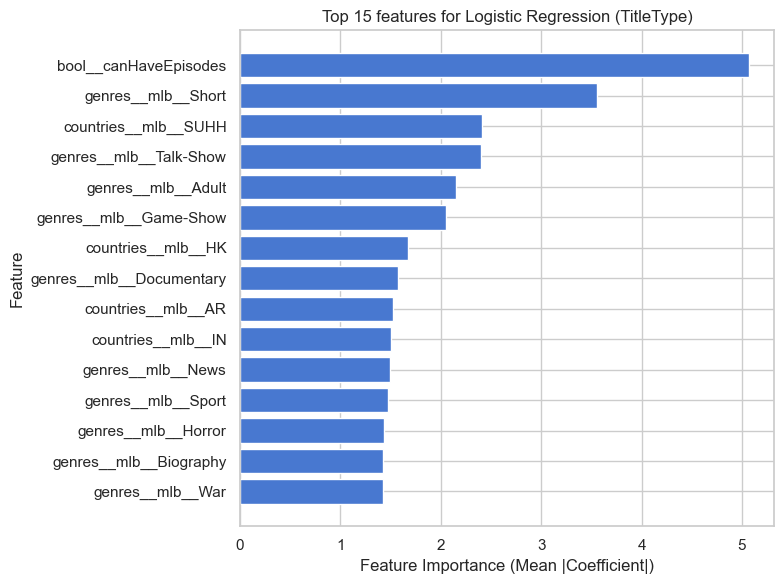
\includegraphics[width=\columnwidth]{../results/images/LR_feat_impo_tt.png}
    \caption{Top 15 most important features for \textit{titleType} (LR).}
    \label{fig:LR_feat_impo_tt.png}
\end{figure}

\subsection{Linear Support Vector Machine}
For Support Vector Machines (SVMs), we scaled numerical features using RobustScaler. We tested the linear kernel and the Radial Basis Function kernel separately to exploit sklearn's optimized LinearSVC implementation.

\subsubsection{Rating}
For LinearSVC, we tested the following parameter grid using a grid search with 5-fold cross validation:

\begin{lstlisting}[basicstyle=\footnotesize\ttfamily,
                   escapeinside={(*@}{@*)}]
  { 'C': [(*@\textbf{0.001}@*), 0.01, 0.1, 1, 10, 100],
    'penalty': ['l1', (*@\textbf{'l2'}@*)],
    'loss': [(*@\textbf{'squared\_hinge'}@*), 'hinge'],
    'max_iter': [5000],
    'class_weight': [None, (*@\textbf{'balanced'}@*)]  }
\end{lstlisting}

It resulted in an average macro F1 of 0.158 for validation and of 0.164 on the training set.

On the test set, w.r.t. Logistic Regression, the model achieved a higher \textbf{macro F1} (\textbf{0.158}), but a lower \textbf{accuracy} (\textbf{0.270}).
Indeed, the F1 for the best performing classes has decreased ((7,8]: 0.496 vs 0.544; (6,7]: 0.215 vs 0.356, (5,6]: 0.259 vs 0.283), in favor of slightly better performances for classes with lower support: the decrease in accuracy is linked to the fact that the model tries to predict these lower support classes more often, rather than focusing merely on the central classes. This led to a notable increase in F1 for (3,4] (0.113 vs 0.04) and (9,10] (0.145 vs 0.046), but it is clear that the model still struggles. The \textbf{PR AUC} is also slightly worse, \textbf{0.175}.

The confusion matrix confirms this tendency: if for Logistic Regression predictions were concentrated on the best performing classes, with many zeros populating the lowest classes, now confusion is spread throughout. 

The most important feature is \textit{tvEpisode} (mean absolute value: 0.175): it is at number one, with negative values, for classes from (2,3] to (5,6] — this would suggest that serialized content is less likely to have bad rating. Classes (7,8] and (8,9] both have \textit{movie} as most important feature, with negative contributions (-0.207 and -190, respectively). This might explain why the latter is mostly classified as the former, which is the class with the highest support.

\subsubsection{Title Type}
The model returned by the grid search yielded an average validation macro F1 of 0.646 (vs 0.654 on the training set); the parameters were \texttt{'C': 0.1, 'class\_weight': 'balanced', 'loss': 'squared\_hinge', 'max\_iter': 5000, 'penalty': 'l1'}.

On the test set, the results were slightly lower than Logistic Regression: \textbf{0.640 macro F1}, \textbf{0.889 accuracy}, \textbf{0.674 PR AUC}. Indeed, performances for almost all classes have decreased to some degree, with a remarkable dip in precision for \textit{videogame} (0.486 vs 0.799).

The overall most important features are the same (\textit{canHaveEpisodes} and genre \textit{Short}), but now only the first stands out (mean absolute value close to 2.5), while \textit{Short} has a similar value to the rest of the top features, < 1.

Unexpectedly, the most important feature for the \textit{titleType} \textit{short} is now \textit{canHaveEpisodes}, with quite an 'advantage' (coef: -2.18, vs genre \textit{Short} 1.43).

\subsection{Support Vector Machine with Radial Basis Function (RBF)}
The power of SVMs comes at a high computational cost, which is why we only tested one kernel function (RBF) and why we opted for an 80/20 holdout, instead of a k-fold cross-validation, to carry out hyperparameter tuning. We also defined a small hyperparameter grid: 
\begin{lstlisting}[basicstyle=\footnotesize\ttfamily,
                   escapeinside={(*@}{@*)}]
  { 'C': [0.1, 1, 10],
    'gamma': ['scale', 0.01, 0.1],
    'class_weight': [None, 'balanced']  }
\end{lstlisting}

\subsubsection{Rating}
The best model returned by the grid search had the following hyperparameters: \texttt{{'C': 10, 'gamma': 0.1, 'class\_weight': None}}. It achieved a macro F1 of 0.265 on the validation set and of 0.698 on the training set, suggesting overfitting.
We therefore reran the grid search, excluding the highest values for C and gamma in order to increase regularization. The best performing model was less overfitted, but also achieved lower results (macro F1 0.206 for validation and 0.316 for training). Its parameters are: \texttt{'C': 1, 'class\_weight': 'balanced', 'gamma': 'scale'}.

On the test set, the overfitted model proved to be the best one, achieving a \textbf{macro F1} of \textbf{0.257} (vs 0.219) and an \textbf{accuracy} of \textbf{0.431} (vs 0.314). The resulting \textbf{PR AUC }is \textbf{0.231}. This model is also the best performing one thus far, with improvements observed across almost all classes.

Looking at the confusion matrix, we can see that the model doesn't completely snub lower support classes, like Logistic Regression did, but is more accurate than LinearSVC. Especially for the more popular (and better performing) classes, confusion is mostly among neighboring classes.

\subsubsection{Title Type}
Similarly to what had happened with \textit{rating}, the first grid search returned an overfitted model (macro F1 for validation: 0.746, vs for training: 0.905). Forcing regularization resulted in less overfitting, but also in a much poorer performance (validation macro F1: 0.206, train macro F1: 0.316); for this reason, we chose the first classifier. Its parameters are: \texttt{'C': 10, 'class\_weight': None, 'gamma': 'scale'}.

On the test set, this model clears all previous attempts, with a \textbf{macro F1} of \textbf{0.746} and an \textbf{accuracy} of \textbf{0.938}.

The performances for all classes increased. \textit{tvEpisode} now achieves an F1 of 0.99; \textit{videogame} improved greatly, reaching 0.884 F1. Nevertheless, we only get a \textbf{PR AUC} of \textbf{0.689}; indeed, the curves in Fig. \ref{fig:pr_svm_rbf_tt.png} show how the precision for half of the classes sinks at around 60\% recall. This means that while the model shows excellent performance metrics on a per-class basis, it has difficulty maintaining a reliable performance when attempting to comprehensively identify instances of minority classes.

\begin{figure}
    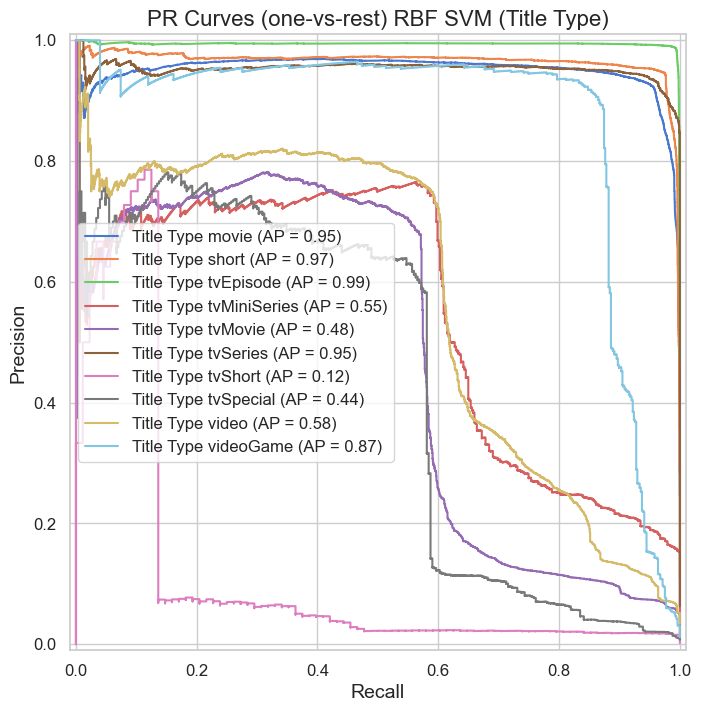
\includegraphics[width=\columnwidth]{../results/images/pr_svm_rbf_tt.png}
    \caption{PR curves for \textit{titleType} (SVM with RBF).}
    \label{fig:pr_svm_rbf_tt.png}
\end{figure}

\subsection{Random Forest}
Since this method is based on trees, no scaling is needed for numerical features. To cut computational costs, we used 3-fold cross validation during hyperparameter tuning.

Indeed, there are many possible hyperparameters to tune. For each task, we ran three Randomized Searches, for a varying number of estimators — 100, 300 and 500, respectively. For each, we tested the same 100 random combinations of parameters from the following grid:
\begin{lstlisting}[basicstyle=\footnotesize\ttfamily,
                   escapeinside={(*@}{@*)}]
  { 'criterion': ["gini", "entropy"],
    'max_depth': [None, 5, 15, 25],
    'min_samples_split': [2, 5, 10],
    'min_samples_leaf': [1, 5, 10],
    'class_weight': [None, 'balanced']  }
\end{lstlisting}

\subsubsection{Rating}
Before proceeding with hyperparameter tuning, we first tested a Random Forest using default parameters, which yielded an average validation macro F1 of 0.296, and an even better 0.302 macro F1 score on the test set.

As shown in Fig. \ref{fig:rf_comparison_n_estimators_rating.png}, the number of estimators is not a strong driver of performance. Although the performance of the other two models was very close, we chose the best model with 300 base classifiers, which yielded an average macro F1 equal to 0.308 for validation, and equal to 0.968 for train. Its parameters are: \texttt{{'n\_estimators': 300, 'min\_samples\_split': 5, 'min\_samples\_leaf': 1, 'max\_depth': None, 'criterion': 'gini', 'class\_weight': 'balanced'}}.

\begin{figure}
    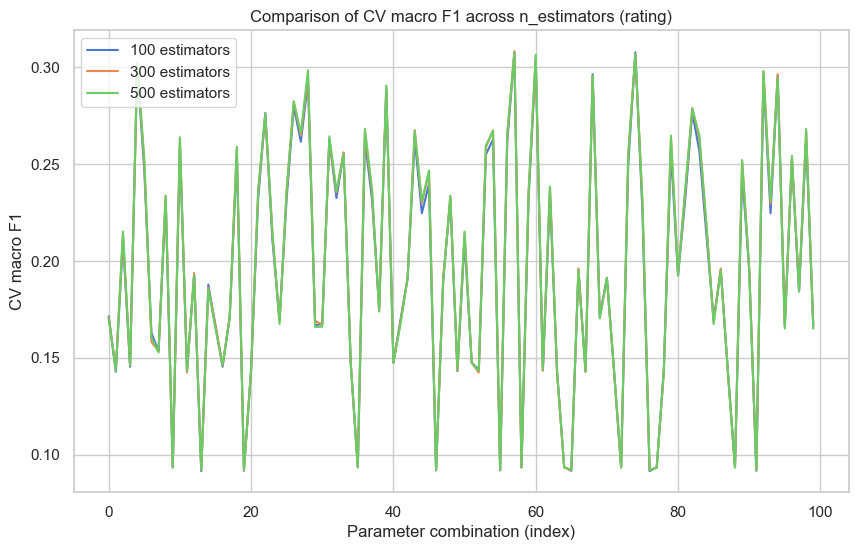
\includegraphics[width=\columnwidth]{../results/images/rf_comparison_n_estimators_rating.png}
    \caption{Avg cross-validation macro F1 for different parameter configurations across varying numbers of estimators for \textit{rating} (RF).}
    \label{fig:rf_comparison_n_estimators_rating.png}
\end{figure}


Whether such a gap between validation and train macro F1 should be seen as a sign of overfitting for Random Forest is debated in the literature: it has been argued that, even if the single trees can overfit, they tend to do so in different ways, and that combining them in an ensemble reduces the overall variance. Thus, although pruning the individual trees can be beneficial, unless the dataset is very simple, we could consider Random Forest as particularly robust against overfitting.

The model's performance on the test set increases, making it the best model thus far: it achieves a \textbf{macro F1} of \textbf{0.325}, an \textbf{accuracy} of \textbf{0.452}, and a \textbf{PR AUC} of \textbf{0.318}.

It achieves the most balanced performance, with six classes out of ten scoring an F1 >= 0.3. Confusion remains spread out for the minority classes (from 0 to 4), whereas for the others it remains concentrated amongst neighboring classes.

The Mean Decrease in Impurity (MDI) returned as the most important features \textit{numVotes} and startYear (almost 0.10), followed by \textit{totalCredits} (around 0.9).

\subsubsection{Title Type}
The default model achieved an average macro F1 of 0.707 on validation and a score of 0.728 on the test set.

The performances for the different parameters combinations tested during the Random Searches were again very similar, with the configurations using 100 estimators yielding marginally lower scores. Indeed, the three best models shared the same hyperparameter values. We chose the configuration with 300 trees: the validation performances were only marginally better than that of the 500-trees model, but we also favored simplicity.

The model yielded 0.767 and 0.975 for validation and training, respectively. Its hyperparameter configuration is the following: \texttt{'n\_estimators': 300, 'min\_samples\_split': 10, 'min\_samples\_leaf': 1, 'max\_depth': None, 'criterion': 'entropy', 'class\_weight': 'balanced'}. 

On the test set, it clears previous models, achieving \textbf{0.777 macro F1} and \textbf{0.940 accuracy}. Half of the classes yield F1 > 0.95. It generalizes better on the minority classes \textit{tvMovie} and \textit{tvMiniSeries}: although there is still confusion with the more popular \textit{movie} and \textit{tvSeries}, they are correctly classified most of the time (cf. the confusion matrix in Fig. \ref{fig:rf_conf_matrix_tt.png}).

This model's superiority across decision thresholds is supported by the PR curves in Fig. \ref{fig:rf_pr_curves.png}, and further quantified by its \textbf{PR AUC} of \textbf{0.818}.

\begin{figure}
    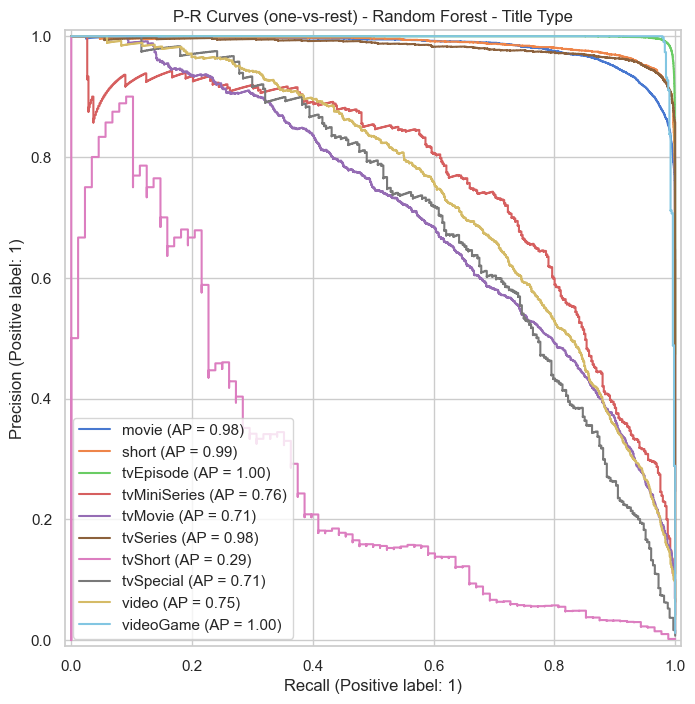
\includegraphics[width=\columnwidth]{../results/images/rf_pr_curves.png}
    \caption{PR curves for \textit{titleType} (RF).}
    \label{fig:rf_pr_curves.png}
\end{figure}

\begin{figure}
    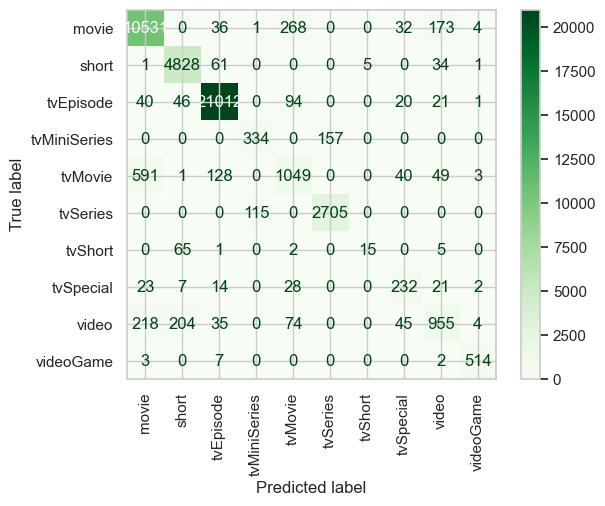
\includegraphics[width=\columnwidth]{../results/images/rf_conf_matrix_tt.png}
    \caption{Confusion matrix for \textit{titleType} (RF).}
    \label{fig:rf_conf_matrix_tt.png}
\end{figure}

Checking the 15 most important features (Fig \ref{fig:rf_feat_impo_tt.png}), we see how the two most important features for the Logistic Regression model, \textit{canHaveEpisodes} and the genre \textit{Short}, have been overtaken by \textit{runtimeMinutes}. Indeed, we had uncovered a relationship between \textit{runtimeMinutes} and \textit{titleType} in Subsec. \ref{handling_nan}.

\begin{figure}
    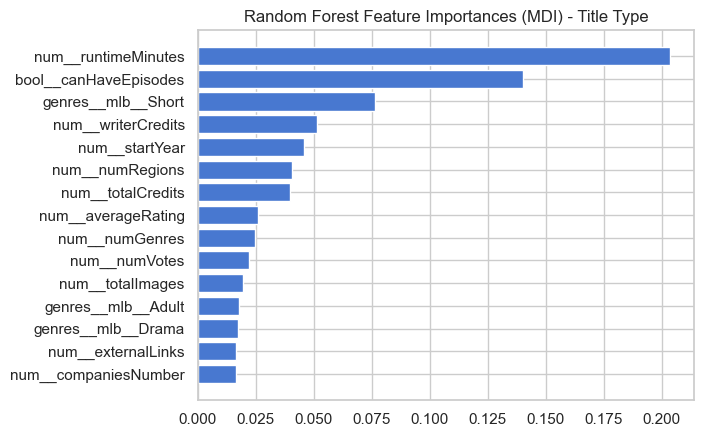
\includegraphics[width=\columnwidth]{../results/images/rf_feat_impo_tt.png}
    \caption{Top 15 most important features for \textit{titleType} (RF).}
    \label{fig:rf_feat_impo_tt.png}
\end{figure}

Finally, it's worth pointing out that prior experimentation keeping the default hyperparameter \texttt{'class\_weight': None} instead of \texttt{'balanced'} lead to a best model scoring a significantly lower macro F1 score of 0.728. This is indicative of the importance of this hyperparameter for this unbalanced task.

\subsection{LightGBM}


\subsection{Multilayer Perceptron}


\subsection{Conclusions}